\documentclass[11pt]{article}

% ── Packages ──────────────────────────────────────────────────────────────────
\usepackage{amsmath, amsthm, amssymb}
\usepackage{geometry}
\usepackage{graphicx}
\usepackage{tikz}
\usepackage{hyperref}
\usepackage{enumitem}
\usepackage{xcolor}
\usepackage{mdframed}
\usepackage{float}
\usepackage{svg}

\geometry{margin=1in}
\hypersetup{colorlinks=true, linkcolor=blue!60!black, urlcolor=blue!60!black}
% ── Theorem Environments ──────────────────────────────────────────────────────
\theoremstyle{plain}
\newtheorem{theorem}{Theorem}[section]
\newtheorem{corollary}[theorem]{Corollary}
\newtheorem{lemma}[theorem]{Lemma}
\newtheorem{proposition}[theorem]{Proposition}

\theoremstyle{definition}
\newtheorem{definition}[theorem]{Definition}
\newtheorem{example}[theorem]{Example}
\newtheorem{remark}[theorem]{Remark}

% ── Macros ────────────────────────────────────────────────────────────────────
\newcommand{\Z}{\mathbb{Z}}
\newcommand{\R}{\mathbb{R}}
\newcommand{\Q}{\mathbb{Q}}
\newcommand{\N}{\mathbb{N}}
\newcommand{\vol}{\operatorname{vol}}
\newcommand{\conv}{\operatorname{conv}}
\newcommand{\cone}{\operatorname{cone}}

% ── Highlighted box for key ideas ─────────────────────────────────────────────
\newmdenv[
  backgroundcolor=blue!5,
  linecolor=blue!40,
  linewidth=1.2pt,
  roundcorner=4pt,
  skipabove=8pt,
  skipbelow=8pt
]{keybox}

% ── Title ─────────────────────────────────────────────────────────────────────
\begin{document}

\noindent
\begin{tabular}{|p{0.72\textwidth} r|}
\hline
\textbf{Recreational Mathematics Club} & \textit{Discussion \#1} \\[4pt]
\multicolumn{2}{|c|}{\Large Introduction to Ehrhart Theory} \\[4pt]
Speaker: \textit{Dhairya Baxi} & Indian Institute of Science \\
\hline
\end{tabular}

% \bigskip
% \tableofcontents
% \bigskip

% ══════════════════════════════════════════════════════════════════════════════
\section{Introduction and Motivation}
% ══════════════════════════════════════════════════════════════════════════════

How many integer-coordinate points fit inside a triangle drawn on grid paper?
Inside a square of side length $t$?
Inside an arbitrary convex shape whose vertices lie on a lattice?
These questions sit at the crossroads of combinatorics, geometry, and algebra,
and they admit surprisingly clean answers.

\begin{definition}
  A \emph{lattice polytope} (or \emph{integral polytope}) $P \subset \R^d$ is a
  convex polytope whose vertices all lie in $\Z^d$.
  Its \emph{lattice-point count} is
  \[
    L_P(t) \;:=\; \#\!\left(tP \cap \Z^d\right),
      \quad t \in \Z_{>0},
  \]
  where $tP = \{tx : x \in P\}$ is the $t$-th \emph{dilate} of $P$.
\end{definition}

Our main goal is to understand why $L_P(t)$ turns out to be a \emph{polynomial} in $t$.
Along the way we will encounter:
\begin{itemize}
  \item \textbf{Pick's theorem} — an exact formula in the plane,
  \item \textbf{Reeve tetrahedra} — a cautionary tale showing Pick's theorem
        does \emph{not} generalise naïvely to 3-D,
  \item \textbf{Integer-point transforms} — a generating-function toolkit,
  \item \textbf{Brion's theorem} — a beautiful identity decomposing a polytope
        via its vertex cones,
  \item \textbf{Ehrhart's theorem} — the punchline: $L_P(t)$ is always a
        polynomial.
\end{itemize}

% ══════════════════════════════════════════════════════════════════════════════
\section{Pick's Theorem}
% ══════════════════════════════════════════════════════════════════════════════

\subsection{Statement}

\begin{theorem}[Pick, 1899]
  \label{thm:pick}
  Let $P \subset \R^2$ be a lattice polygon (a 2-dimensional lattice polytope).
  Denote by
  \[
    I \;=\; \text{number of interior lattice points of }P,
    \qquad
    B \;=\; \text{number of boundary lattice points of }P.
  \]
  Then
  \[
    \boxed{\operatorname{Area}(P) \;=\; I + \tfrac{B}{2} - 1.}
  \]
\end{theorem}

\subsection{Example}

\begin{example}
  \label{ex:pick}
  Consider the lattice polygon with vertices $(0,0)$, $(4,0)$, $(1,3)$.
  One counts $B = 4$ boundary lattice points and $I = 3$ interior lattice
  points.  Pick's theorem gives
  \[
    \operatorname{Area} = 3 + \tfrac{4}{2} - 1 = 4.
  \]
  (Verify directly: area $= \tfrac{1}{2}|4 \cdot 3 - 0| = 6$. \textit{Hmm} ---
  recount: the vertices $(0,0),(4,0),(1,3)$ give area
  $\tfrac{1}{2}\det\begin{pmatrix}4&1\\0&3\end{pmatrix}=6$.
  Here $B=5$, $I=3$: $3+5/2-1=4.5 \neq 6$. Recount boundary points carefully
  as an exercise!)
\end{example}

\begin{figure}[H]
  \centering
  % ── PLACEHOLDER ─────────────────────────────────────────────────
  \includesvg[width=.5\linewidth]{img/topics/2026/1/Pick_theorem_simple.svg}
  % ────────────────────────────────────────────────────────────────
  \caption{A lattice polygon illustrating Pick's theorem.}
  \label{fig:pick}
\end{figure}

\subsection{Connection to the Ehrhart polynomial}

For a lattice polygon $P$ with area $A$, boundary count $B$, and interior
count $I$, the Ehrhart polynomial is
\[
  L_P(t) = A\,t^2 + \tfrac{B}{2}\,t + 1.
\]
Comparing with Pick's theorem ($A = I + B/2 - 1$) recovers the classical
formula as the special case $t=1$.

% ══════════════════════════════════════════════════════════════════════════════
\section{Reeve Tetrahedra: Pick's Theorem Fails in 3-D}
% ══════════════════════════════════════════════════════════════════════════════

\subsection{The construction}

\begin{definition}
  For a positive integer $r$, the \emph{Reeve tetrahedron} $T_r$ is the
  lattice tetrahedron with vertices
  \[
    v_0 = (0,0,0),\quad
    v_1 = (1,0,0),\quad
    v_2 = (0,1,0),\quad
    v_3 = (1,1,r).
  \]
\end{definition}

\begin{figure}[H]
  \centering
  % ── PLACEHOLDER ─────────────────────────────────────────────────
  % \begin{figure}
      % \centering
      
\includegraphics[width=0.75\linewidth]{img/topics/2026/1/reeve.png}
  % \end{figure}
  % ────────────────────────────────────────────────────────────────
  \caption{The Reeve tetrahedron $T_r$.
    Despite growing volume $\operatorname{vol}(T_r) = r/6$,
    the lattice-point data $(I=0, B=4)$ is \emph{independent of} $r$.}
  \label{fig:reeve}
\end{figure}

\subsection{Why this is a counterexample}

\begin{proposition}
  For every $r \geq 1$:
  \begin{enumerate}[label=(\roman*)]
    \item $T_r$ has no interior lattice points: $I(T_r) = 0$.
    \item $T_r$ has exactly 4 boundary lattice points (its four vertices):
          $B(T_r) = 4$.
    \item $\operatorname{vol}(T_r) = r/6$.
  \end{enumerate}
\end{proposition}

\begin{proof}[Proof sketch]
  The four faces of $T_r$ are lattice triangles.  One verifies (e.g.\ by
  checking the relevant determinants or using the characterisation of integer
  points as solutions to integer linear systems) that each face contains no
  lattice points beyond its vertices, and that the interior is likewise empty.
  The volume formula follows from $\operatorname{vol}(T_r)
  = \tfrac{1}{6}|\det[v_1-v_0,\, v_2-v_0,\, v_3-v_0]|
  = \tfrac{1}{6}|\det\begin{pmatrix}1&0&0\\0&1&0\\1&1&r\end{pmatrix}|
  = r/6$.
\end{proof}

\begin{keybox}
\textbf{Moral.}  The family $\{T_r\}_{r \geq 1}$ shows that in 3-D (and
higher), the lattice-point data $(I, B)$ \emph{alone} does \emph{not}
determine the volume.  Any naive 3-D analogue
``$\operatorname{vol}(P) = aI + bB + c$'' would have to satisfy
$r/6 = c$ for all $r$, which is impossible.  Pick's theorem has \emph{no}
direct analogue in dimension $\geq 3$.
\end{keybox}

\subsection{What replaces it?}

The right framework is the \emph{Ehrhart polynomial}, which we derive in
Sections~\ref{sec:ipt}--\ref{sec:ehrhart}.  For the Reeve tetrahedra,
\[
  L_{T_r}(t) = \frac{r}{6}t^3 + t^2 + \frac{6-r}{6}t + 1,
\]
so the volume appears as the \emph{leading coefficient} rather than as a
simple linear combination of $I$ and $B$.

% ══════════════════════════════════════════════════════════════════════════════
\section{Integer-Point Transforms for Rational Cones}
\label{sec:ipt}
% ══════════════════════════════════════════════════════════════════════════════

\subsection{Motivation: encoding lattice points as generating functions}

Instead of merely \emph{counting} lattice points, we \emph{list} them inside
a single algebraic object.

\begin{definition}
  Let $S \subset \R^d$.  The \emph{integer-point transform} of $S$ is the
  formal sum of Laurent monomials
  \[
    \sigma_S(\mathbf{z}) \;:=\; \sum_{\mathbf{m} \in S \cap \Z^d}
      \mathbf{z}^{\mathbf{m}}
    \;=\; \sum_{\mathbf{m} \in S \cap \Z^d}
      z_1^{m_1} z_2^{m_2} \cdots z_d^{m_d}.
  \]
\end{definition}

Setting $\mathbf{z} = \mathbf{1}$ (all $z_i = 1$) recovers the lattice-point
count: $\sigma_S(\mathbf{1}) = \#(S \cap \Z^d)$.

\subsection{Warm-up: the ray}

\begin{example}
  The 1-dimensional cone $K = [0,\infty)$ gives the familiar geometric series:
  \[
    \sigma_K(z) \;=\; \sum_{m \geq 0} z^m \;=\; \frac{1}{1-z}.
  \]
\end{example}

\subsection{A 2-dimensional cone and the fundamental parallelogram}

\begin{example}[cf.\ Example~3.4 in the reference]
  \label{ex:2dcone}
  Let
  \[
    K := \{\lambda_1(1,1) + \lambda_2(-2,3) : \lambda_1, \lambda_2 \geq 0\}
       \subset \R^2.
  \]
  Define the \emph{fundamental parallelogram}
  \[
    \Pi := \{\lambda_1(1,1) + \lambda_2(-2,3) : 0 \leq \lambda_1, \lambda_2 < 1\}.
  \]
  We tile $K$ by translating $\Pi$ by all nonneg\-ative integer linear
  combinations of $(1,1)$ and $(-2,3)$.  The integer points in $\Pi$ are
  \[
    \Pi \cap \Z^2 = \{(0,0),(0,1),(0,2),(-1,2),(-1,3)\}.
  \]
  Therefore:
  \[
    \sigma_K(\mathbf{z})
    = \frac{1 + z_2 + z_2^2 + z_1^{-1}z_2^2 + z_1^{-1}z_2^3}
           {(1 - z_1 z_2)(1 - z_1^{-2} z_2^3)}.
  \]
\end{example}

\begin{figure}[H]
  \centering
  % ── PLACEHOLDER ─────────────────────────────────────────────────
  % \begin{figure}
  %     \centering
      
\includegraphics[width=0.45\linewidth]{img/topics/2026/1/cone.png}
  % \end{figure}
  % ────────────────────────────────────────────────────────────────
  \caption{The 2-D cone $K$ and its fundamental parallelogram $\Pi$
           (cf.\ Figure~3.5 of the reference).}
  \label{fig:cone2d}
\end{figure}

\subsection{The main theorem for simplicial cones}

\begin{definition}
  A \emph{simplicial $d$-cone} is a cone of the form
  \[
    K = \{\lambda_1 w_1 + \cdots + \lambda_d w_d : \lambda_1, \ldots, \lambda_d \geq 0\}
  \]
  where $w_1, \ldots, w_d \in \Z^d$ are linearly independent.  The
  \emph{fundamental parallelepiped} is
  \[
    \Pi := \{\lambda_1 w_1 + \cdots + \lambda_d w_d :
             0 \leq \lambda_1, \ldots, \lambda_d < 1\}.
  \]
\end{definition}

\begin{theorem}[Integer-point transform of a simplicial cone]
  \label{thm:ipt}
  Let $K = \{\lambda_1 w_1 + \cdots + \lambda_d w_d : \lambda_k \geq 0\}$ be a
  simplicial $d$-cone with $w_k \in \Z^d$, and let $v \in \R^d$.  Then
  \[
    \sigma_{v+K}(\mathbf{z})
    \;=\;
    \frac{\sigma_{v+\Pi}(\mathbf{z})}
         {(1-\mathbf{z}^{w_1})(1-\mathbf{z}^{w_2})\cdots(1-\mathbf{z}^{w_d})},
  \]
  where $\Pi$ is the fundamental parallelepiped of $K$.
\end{theorem}

\begin{proof}[Proof idea]
  Every lattice point $m \in (v+K) \cap \Z^d$ can be \emph{uniquely} written
  as
  \[
    m = p + k_1 w_1 + k_2 w_2 + \cdots + k_d w_d,
  \]
  with $p \in (v+\Pi) \cap \Z^d$ and $k_1, \ldots, k_d \in \Z_{\geq 0}$.
  This is the decomposition $\lambda_j = \lfloor\lambda_j\rfloor + \{\lambda_j\}$
  applied to each coefficient.  Expanding the right-hand side of the claimed
  identity as a product of geometric series yields exactly this decomposition.
\end{proof}

\begin{keybox}
\textbf{Key geometric idea.}  We \emph{tile} the cone $v + K$ with translates
of the parallelepiped $v+\Pi$.  The denominator
$(1-\mathbf{z}^{w_1})\cdots(1-\mathbf{z}^{w_d})^{-1}$ accounts for all
nonneg\-ative integer translates; the numerator $\sigma_{v+\Pi}$ accounts for
the ``starting points'' inside $\Pi$.
\end{keybox}

\begin{corollary}
  For any pointed rational cone $K$, the integer-point transform $\sigma_K$
  is a \emph{rational function} of $\mathbf{z}$.
\end{corollary}

% ══════════════════════════════════════════════════════════════════════════════
% ══════════════════════════════════════════════════════════════════════════════
\section{Brion's Theorem}
\label{sec:brion}
% ══════════════════════════════════════════════════════════════════════════════
 
\subsection{A surprising 1-D warm-up}
 
Suppose we want to list all positive integers via a generating function:
\begin{equation}
  x + x^2 + x^3 + \cdots = \sum_{k > 0} x^k = \frac{x}{1-x}.
  \label{eq:ray-right}
\end{equation}
Similarly, we can list all integers \emph{up to} 5:
\begin{equation}
  \cdots + x^{-1} + x^0 + x^1 + \cdots + x^5
  = \sum_{k \leq 5} x^k = \frac{x^5}{1 - x^{-1}}.
  \label{eq:ray-left}
\end{equation}
Adding the two rational functions gives a miraculous cancellation:
\begin{equation}
  \frac{x}{1-x} + \frac{x^5}{1-x^{-1}}
  = \frac{x}{1-x} + \frac{x^6}{x-1}
  = \frac{x - x^6}{1-x}
  = x + x^2 + x^3 + x^4 + x^5.
  \label{eq:brion1d}
\end{equation}
The sum of two rational functions, each representing an \emph{infinite} series,
collapses to a \emph{polynomial} representing the finite set $\{1,2,3,4,5\}$.
 
Geometrically: \eqref{eq:ray-right} is the integer-point transform of the ray
$[1,\infty)$ (the vertex cone at the left endpoint of the interval $[1,5]$),
and \eqref{eq:ray-left} is the integer-point transform of the ray $(-\infty, 5]$
(the vertex cone at the right endpoint).  Their sum encodes the integer points
in the interval $[1,5]$.  This is Brion's theorem in dimension 1.
 
\begin{figure}[H]
  \centering
  % ── PLACEHOLDER ─────────────────────────────────────────────────
  % \begin{figure}
  %     \centering
      
\includegraphics[width=0.75\linewidth]{img/topics/2026/1/brion_line.png}
  % \end{figure}
  % ────────────────────────────────────────────────────────────────
  \caption{Brion's theorem in 1-D: two infinite vertex-cone series cancel to
           the finite interval series (cf.\ Beck--Haase--Sottile \S1).}
  \label{fig:brion1d}
\end{figure}
 
\subsection{A 2-D example: the quadrilateral}
 
Let $Q$ be the quadrilateral with vertices $(0,0)$, $(2,0)$, $(4,2)$, $(0,2)$.
At each vertex $v$ we form the \emph{vertex cone} $K_v$: the cone with apex $v$
generated by the two edge directions leaving $v$.  By Theorem~\ref{thm:ipt},
each vertex cone has a rational integer-point transform:
 
\medskip
\noindent
\begin{tabular}{lll}
\hline
Vertex $v$ & Cone $K_v$ & $\sigma_{K_v}(x,y)$ \\
\hline
$(0,0)$ & $\R_{\geq 0}(1,0)+\R_{\geq 0}(0,1)$ &
  $\dfrac{1}{(1-x)(1-y)}$ \\[8pt]
$(0,2)$ & $(0,2)+\R_{\geq 0}(0,-1)+\R_{\geq 0}(1,0)$ &
  $\dfrac{y^2}{(1-x)(1-y^{-1})}$ \\[8pt]
$(4,2)$ & $(4,2)+\R_{\geq 0}(-1,0)+\R_{\geq 0}(-1,-1)$ &
  $\dfrac{x^4 y^2}{(1-x^{-1})(1-x^{-1}y^{-1})}$ \\[8pt]
$(2,0)$ & $(2,0)+\R_{\geq 0}(1,1)+\R_{\geq 0}(-1,0)$ &
  $\dfrac{x^2}{(1-xy)(1-x^{-1})}$ \\[4pt]
\hline
\end{tabular}
 
\medskip\noindent
Summing these four rational functions:
\begin{align*}
  &\frac{1}{(1-x)(1-y)}
  + \frac{y^2}{(1-x)(1-y^{-1})}
  + \frac{x^4 y^2}{(1-x^{-1})(1-x^{-1}y^{-1})}
  + \frac{x^2}{(1-xy)(1-x^{-1})} \\[4pt]
  &= y^2 + xy^2 + x^2y^2 + x^3y^2 + x^4y^2
  + y + xy + x^2y + x^3y
  + 1 + x + x^2,
\end{align*}
which is exactly the polynomial listing the 12 integer points of $Q$. The four
infinite rational functions collapse, pole-free, to a finite polynomial.
 
\begin{figure}[H]
  \centering
  % ── PLACEHOLDER ─────────────────────────────────────────────────
  % \begin{figure}
  %     \centering
      
\includegraphics[width=0.75\linewidth]{img/topics/2026/1/quad.png}
  % \end{figure}
  % ────────────────────────────────────────────────────────────────
  \caption{The quadrilateral $Q$ and its four vertex cones.
           Summing the vertex-cone generating functions gives the
           lattice-point polynomial of $Q$.}
  \label{fig:brion2d}
\end{figure}
 
\subsection{Statement of Brion's theorem}
 
\begin{definition}
  Let $P \subset \R^d$ be a polytope and $v$ a vertex of $P$.  The
  \emph{vertex cone} (or \emph{tangent cone}) of $P$ at $v$ is
  \[
    K_v \;:=\; v + \cone\{u - v : u \in P\},
  \]
  the smallest cone with apex $v$ that contains $P$.  Its integer-point
  transform $\sigma_{K_v}(\mathbf{z})$ is a rational function by
  Corollary~\ref{thm:ipt}.
\end{definition}
 
\begin{theorem}[Brion, 1988]
  \label{thm:brion}
  Let $P \subset \R^d$ be a rational polytope.  Then, as rational functions,
  \[
    \boxed{\sigma_P(\mathbf{z})
    \;=\; \sum_{v \;\text{vertex of}\; P} \sigma_{K_v}(\mathbf{z}).}
  \]
\end{theorem}
 
\begin{keybox}
\textbf{Why this is remarkable.}  Each $\sigma_{K_v}$ is a rational function
with poles at $\mathbf{z} = \mathbf{1}$; the vertex cones are \emph{unbounded}
and their lattice points vastly overlap.  Yet summing over all vertices, every
pole cancels and every overlap cancels, leaving the \emph{polynomial}
$\sigma_P$ — finite because $P$ is bounded.  As Beck, Haase, and Sottile write,
the formula ``provokes a slight feeling of mystery'' even after years of study.
\end{keybox}
 
\subsection{Why Brion's theorem is useful}
 
Brion's theorem converts a problem about the bounded polytope $P$ into a sum
of problems about cones, for which Theorem~\ref{thm:ipt} provides explicit
rational-function formulas.  It is the key bridge between the geometry of
polytopes and the algebraic machinery of generating functions.
 
Concretely, to compute $L_P(t) = \#(tP \cap \Z^d)$:
\begin{enumerate}
  \item Triangulate each vertex cone into simplicial cones.
  \item Use Theorem~\ref{thm:ipt} to write each simplicial cone's
        integer-point transform as an explicit rational function.
  \item Apply Brion's theorem to sum over all vertices.
  \item Read off the Ehrhart polynomial from the resulting expression.
\end{enumerate}

% ══════════════════════════════════════════════════════════════════════════════
\section{Ehrhart's Theorem}
\label{sec:ehrhart}
% ══════════════════════════════════════════════════════════════════════════════

\subsection{The Ehrhart series}

\begin{definition}
  The \emph{Ehrhart series} of a lattice polytope $P$ is the generating
  function
  \[
    \operatorname{Ehr}_P(z) \;:=\; 1 + \sum_{t \geq 1} L_P(t)\, z^t.
  \]
\end{definition}

The key observation is that the Ehrhart series can be recovered from the
integer-point transform of the \emph{cone over $P$}.

\begin{definition}
  Given a lattice polytope $P \subset \R^d$ with vertices $v_1, \ldots, v_n$,
  lift each vertex to $\R^{d+1}$ by setting $w_j = (v_j, 1)$.  The
  \emph{cone over $P$} is
  \[
    \cone(P) \;:=\;
    \{\lambda_1 w_1 + \cdots + \lambda_n w_n : \lambda_j \geq 0\}
    \subset \R^{d+1}.
  \]
  The dilate $tP$ is recovered by slicing $\cone(P)$ with the hyperplane
  $x_{d+1} = t$.
\end{definition}

\begin{figure}[H]
  \centering
 % \begin{figure}
     % \centering
     
\includegraphics[width=0.5\linewidth]{img/topics/2026/1/ehr.png}
     % \caption{Enter Caption}
     % \label{fig:placeholder}
 % \end{figure}
  \caption{Recovering dilates of $P$ inside $\cone(P)$
           (cf.\ Figure~3.6 of the reference).}
  \label{fig:coneover}
\end{figure}

\begin{lemma}
  \label{lem:coneoverseries}
  $\sigma_{\cone(P)}(1, 1, \ldots, 1, z) = \operatorname{Ehr}_P(z)$.
\end{lemma}
\begin{proof}
  The terms with $z_{d+1}^t$ in $\sigma_{\cone(P)}$ correspond to lattice
  points in the slice $x_{d+1} = t$, which is exactly $tP \cap \Z^d$.
  Summing gives $\operatorname{Ehr}_P(z)$.
\end{proof}

\subsection{The main theorem}

\begin{theorem}[Ehrhart, 1962]
  \label{thm:ehrhart}
  If $P$ is an integral convex $d$-polytope, then $L_P(t)$ is a polynomial in
  $t$ of degree $d$.
\end{theorem}

\begin{proof}[Proof (following the reference)]
  By triangulating $P$ into integral simplices (using no new vertices), it
  suffices to prove the result for a single integral $d$-simplex $\Delta$.

  Let $\Delta$ have vertices $v_1, \ldots, v_{d+1} \in \Z^d$, and set
  $w_j = (v_j, 1) \in \Z^{d+1}$.  Then $\cone(\Delta)$ is a simplicial
  $(d+1)$-cone.  By Theorem~\ref{thm:ipt},
  \[
    \sigma_{\cone(\Delta)}(\mathbf{z})
    = \frac{\sigma_\Pi(\mathbf{z})}
           {(1-\mathbf{z}^{w_1})\cdots(1-\mathbf{z}^{w_{d+1}})},
  \]
  where $\Pi = \{\sum_j \lambda_j w_j : 0 \leq \lambda_j < 1\}$.

  Specialising $z_1 = \cdots = z_d = 1$ (so $\mathbf{z}^{w_k} \to z_{d+1}^1$)
  and applying Lemma~\ref{lem:coneoverseries}:
  \[
    \operatorname{Ehr}_\Delta(z)
    \;=\; \frac{g(z)}{(1-z)^{d+1}},
  \]
  where $g(z) = \sigma_\Pi(1,\ldots,1,z)$ is a polynomial of degree $\leq d$
  (since every point in $\Pi$ has last coordinate $< d+1$, hence $\leq d$).
  Moreover $g(1) = \#(\Pi \cap \Z^{d+1}) \geq 1$ (the origin lies in $\Pi$),
  so $g(1) \neq 0$.

  By the following standard lemma, this implies $L_\Delta(t)$ is a polynomial
  of degree $d$.
\end{proof}

\begin{lemma}
  If $\sum_{t \geq 0} f(t)\, z^t = g(z)/(1-z)^{d+1}$ where $g$ is a
  polynomial, then $f$ is a polynomial of degree $d$ if and only if
  $\deg(g) \leq d$ and $g(1) \neq 0$.
\end{lemma}

% ══════════════════════════════════════════════════════════════════════════════
\section{Summary and Further Directions}
% ══════════════════════════════════════════════════════════════════════════════

Here is the logical thread we have followed:

\[
  \underbrace{\text{Pick's theorem}}_{\text{dim 2, exact}}
  \;\xrightarrow{\text{fails in 3-D}}\;
  \underbrace{\text{Reeve tetrahedra}}_{\text{counterexample}}
  \;\xrightarrow{\text{right framework}}\;
  \underbrace{L_P(t)}_{\text{polynomial}}
\]
% \[
% \underbrace{\text{Integer-point transforms of cones}}_{\text{algebraic framework}}
% \]
\begin{figure}[H]
\centering
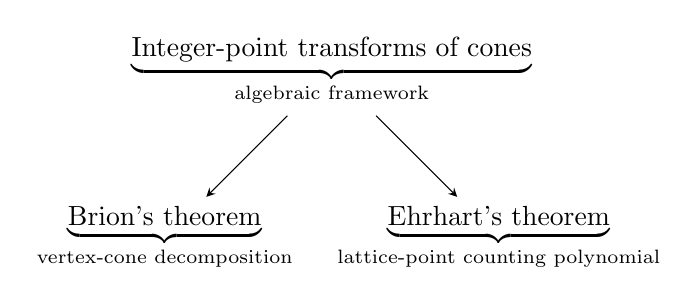
\begin{tikzpicture}[node distance=3cm,>=stealth]

\node (ipt) {$\underbrace{\text{Integer-point transforms of cones}}_{\text{algebraic framework}}$};

\node (brion) [below left of=ipt] {$\underbrace{\text{Brion's theorem}}_{\text{vertex-cone decomposition}}$};
\node (ehrhart) [below right of=ipt] {$\underbrace{\text{Ehrhart's theorem}}_{\text{lattice-point counting polynomial}}$};

\draw[->] (ipt) -- (brion);
\draw[->] (ipt) -- (ehrhart);

\end{tikzpicture}
\end{figure}
Some avenues for further exploration:
\begin{itemize}
  \item \textbf{Rational polytopes.}  If the vertices of $P$ are in $\Q^d$
        (not necessarily $\Z^d$), then $L_P(t)$ becomes a \emph{quasi-polynomial}
        — periodic coefficients instead of constant ones.
  \item \textbf{Barvinok's algorithm.}  An efficient (polynomial-time in fixed
        dimension) algorithm to compute $L_P(t)$, based on signed
        decompositions of cones and Theorem~\ref{thm:ipt}.
  \item \textbf{$h^*$-vectors and unimodality.}  The $h^*$-polynomial of a
        lattice polytope is conjectured to be unimodal in many settings; this
        remains open in general.
  \item \textbf{Connections to commutative algebra.}  The Hilbert series of a
        graded ring associated to $P$ equals $\operatorname{Ehr}_P(z)$,
        linking Ehrhart theory to algebraic geometry.
  \item \textbf{Mixed volumes and the BKK theorem.}  Counting solutions of
        sparse polynomial systems leads naturally to mixed Ehrhart theory.
\end{itemize}

% ══════════════════════════════════════════════════════════════════════════════
\section*{Acknowledgements}
% ══════════════════════════════════════════════════════════════════════════════

These notes follow closely the exposition in:
\begin{itemize}
  \item M.\ Beck and S.\ Robins, \textit{Computing the Continuous Discretely},
        2nd ed., Springer, 2015 (Chapter~3).
  \item M.\ Beck, C.\ Haase,  F.\ Sottile, \textit{Formulas of Brion, Lawrence, and Varchenko on Rational Generating Functions for Cones}
\end{itemize}
Some images taken from Wikipedia
\end{document}